\section{Data \& Methods}\label{sec:methods}

\hspace{13pt} This study makes use of data scraped from an online repository of open-source statistical software. All scraping and analysis scripts are freely availably online.\footnote{Source code is available at: \href{https://github.com/simonpcouch/social_divisions_in_data}{\textit{https://github.com/simonpcouch/social\_divisions\_in\_data}}}

\subsection{Data Acquisition}\label{sec:data}

\hspace{13pt} The Comprehensive R Archive Network (CRAN) is a repository of, at the time of writing, over 15,300 open-source statistical software packages for use with the R programming language. In addition to housing code libraries, many of these packages contain data, either serving as the primary purpose of the package or for use in examples showcasing the functionality of the code libraries. Those working with the R language use these libraries in a large variety of contexts, from academic research in biology, social science, and statistics, to commercial applications in finance and data science, to teaching statistics and analytics \cite{hornik2012comprehensive}. I make use of this repository in order to sample datasets used in a variety of contexts---namely, identifying those that are used for biological purposes versus those that are not. I use an automated, algorithmic approach to gather data from CRAN.

Initially, I scraped a list of all packages and relevant metadata such as package descriptions and documentation URLs from CRAN's website logs. 

While CRAN offers a large sample of diverse datasets, and hosts a variety of metadata relevant to this analysis, the repository currently does not systematically classify packages based on their purpose or intent. To address this, I use a two-part approach to infer the purpose of the package. Initially, I utilize CRAN Task Views (CTV), a CRAN-hosted service offering lists of packages curated for carrying out specific tasks (e.g. ``TeachingStatistics'' or  ``ClinicalTrials'') \cite{zeileis2005cran}. I first make use of this service to identify an initial sample of packages in each of the relevant categories. Next, I make use of package metadata to more coarsely infer the purpose of each package. Using narrative description data, packages are sorted using the presence of keywords and phrases. In combining these two data sources, I prioritize the curated CTV classifications---if a package has a classification from CTV, the package is sorted using this grouping. Then, classifiers for the remaining packages are interpolated using the keyword matching procedure. The numbers of packages in each of these groups are shown in Table \ref{tab:n_by_grp}; for computability, I take a sample of packages from the ``Other'' category.

For each package in the sample, the program checks whether the package contains datasets. If it does, it stores the names of each of them. Then, for each dataset in the package, the program searches for matches to several keywords in the column names of the dataset (e.g. ``Sex'' or ``Gender.'') If any of these keywords are matched, an algorithm chooses the column most likely to contain information relevant to the keyword of interest. Finally, the program extracts all unique entries in the column (e.g. a column titled ``Sex'' might contain the unique entries ``Female'' and ``Male,'') and store them in a dataset giving the unique value, the number of times it appeared, the column it appeared as an entry to, the name of the dataset containing the column, and the package containing the dataset. This process is iterated over every keyword, in every column, in every dataset, in every package in the sample. Then, a set of criteria generates a cleaned version of the entries in order to allow for basic text analytics, collapsing values that encode essentially the same value (e.g. ``woman'', ``Woman'', and ``W'' are all encoded as ``Woman.'') Summary statistics about this dataset are presented in Tables \ref{tab:n_by_grp} and \ref{tab:n_columns_by_grp}.

\subsection{Analysis} \label{sec:analysis}

\hspace{13pt} Making use of this data, I develop a set of sub-hypotheses to empirically test the hypotheses given in Section \ref{sec:hyps}.

\begin{itemize}
  \item \textit{Hypothesis 1(a).} Datasets from packages intended for biological purposes will be more likely to refer to sex/gender measures as sex rather than gender, if one or the other is included, than datasets from packages intended for other purposes.
  \item \textit{Hypothesis 1(b).} Datasets from packages intended for biological purposes will be more likely to refer to race/ethnicity measures as race rather than ethnicity, if one or the other is included, than datasets from packages intended for other purposes.
\end{itemize}

To test Hypotheses $1(a)$ and $1(b)$, I use a t-test for difference in proportions. To carry out this procedure to test Hypothesis $1(a)$, I first collect a list of all datasets in the sample, and whether that dataset supplies a column called ``Sex,'' ``Gender,'' or both. Then, I calculate the proportion of datasets for biological purposes that supply a column called ``Sex,'' and the same proportion for datasets that are not for biological purposes. Then, if the difference between the two (former minus the latter) is greater than zero, then packages intended for biological purposes are more likely to refer to sex than gender. The statistical significance of this finding is then tested to assess the validity of the above Hypothesis. A visual representation of the observed data relevant to these hypotheses are shown in Figure \ref{fig:common_names}.

\begin{figure} [!htb]
    \caption{Column Name Choice by Dataset Purpose}
    \centering
    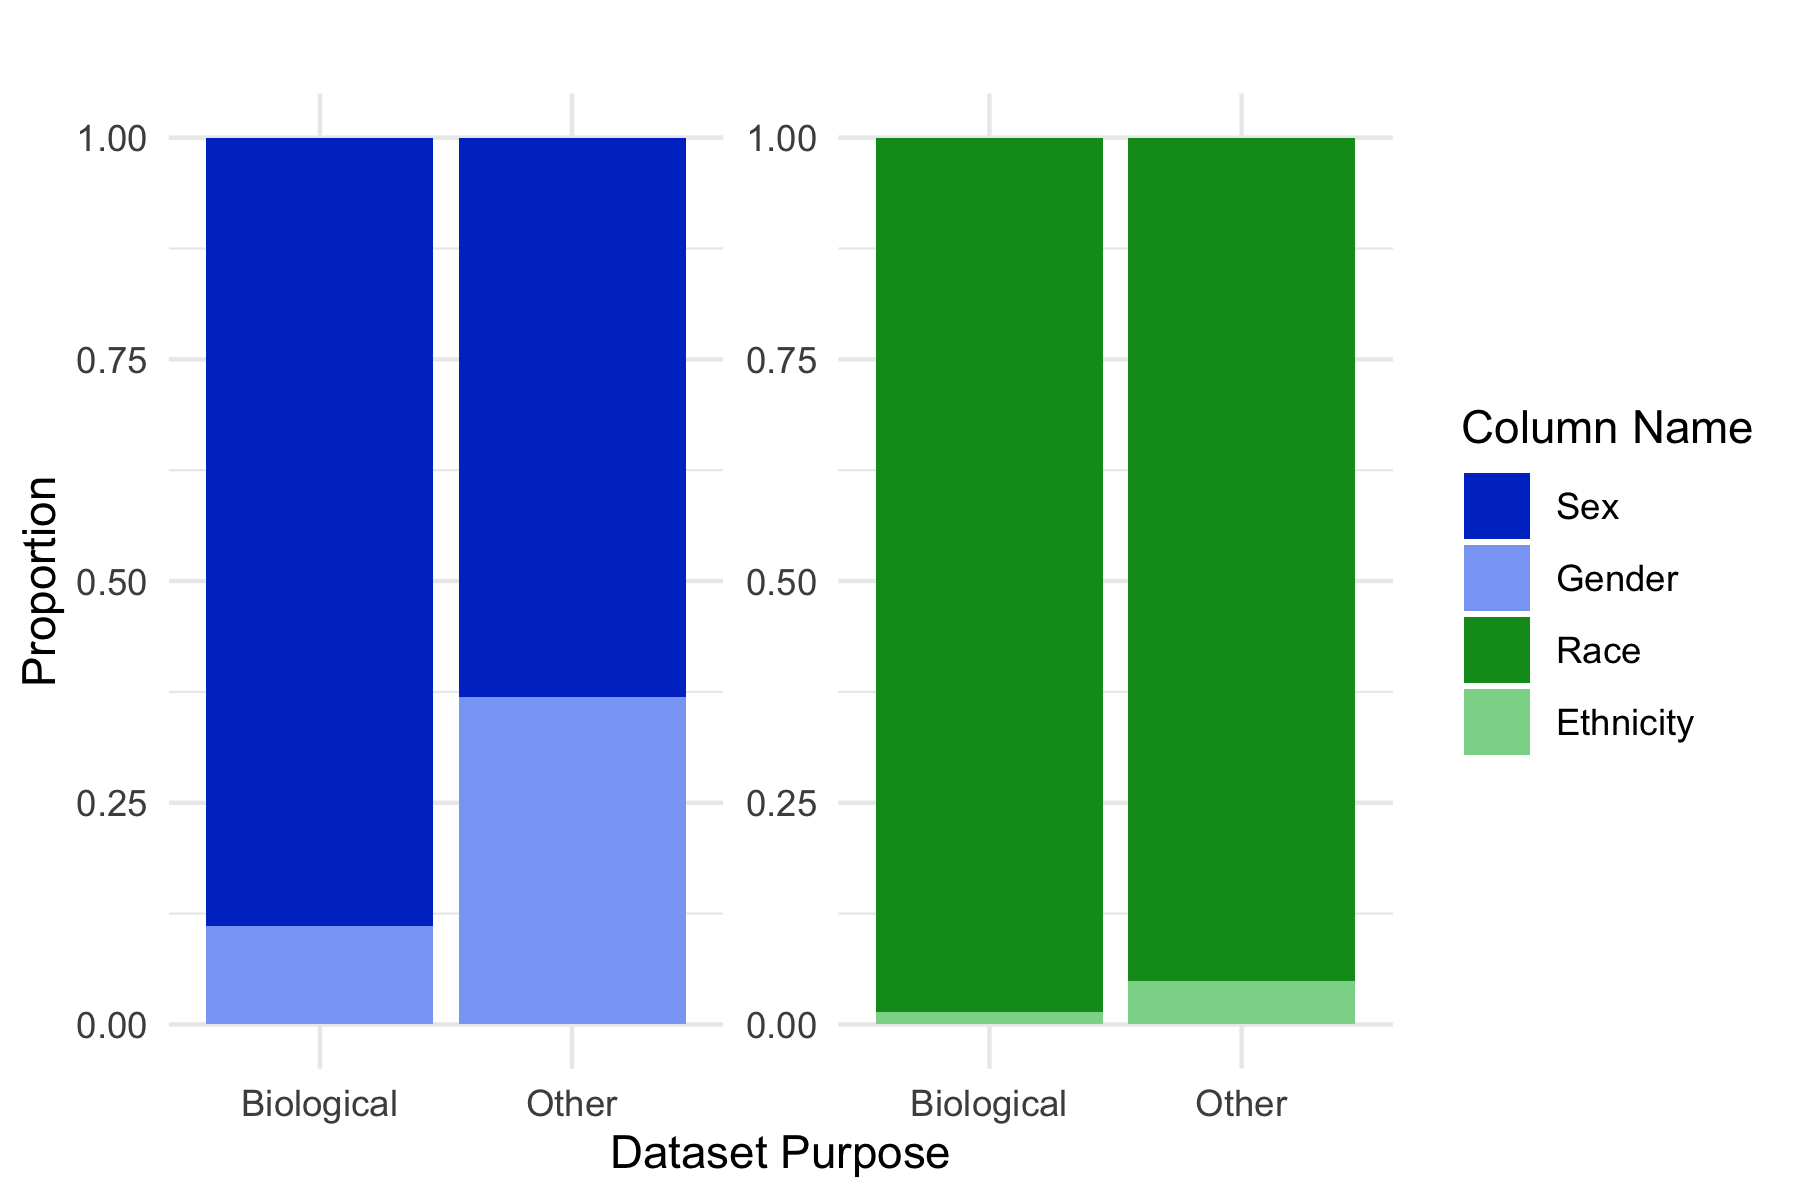
\includegraphics[width=.8\linewidth]{figures/common_names.png}
    \captionsetup{width=0.8\textwidth}
    \caption*{The proportion of columns in datasets for either biological purposes, or some other purpose, named with terms evoking biological or social connotations. The difference in these proportions is tested in evaluating Hypotheses $1(a)$ and $1(b)$. See Table \ref{tab:n_columns_by_grp} for raw data.}
    \label{fig:common_names}
\end{figure}

\begin{itemize}
  \item \textit{Hypothesis 2(a).} The distribution of values in columns named ``Sex’’ will not differ from that of columns named ``Gender.'' Namely, the frequencies of the entries ``Male,'' ``Female,'' and others (as a group) will not be different.
  \item \textit{Hypothesis 2(b).} The distribution of values in columns named ``Race’’ will not differ from that of columns named ``Ethnicity.'' Namely, the frequencies of the entries ``Black,'' ``White,'' and others (as a group) will not be different.
\end{itemize}

Note that all sampled data is used to test this hypothesis, rather than just that inferred to be intended for use in biological contexts. Given the discussion above, this choice should result in greater divergence between the two distributions. This will result in a greater likelihood of statistical significance, which, in this case, leads to a more conservative evaluation of this hypothesis.

In order to test Hypotheses $2(a)$ and $2(b)$, I make use of the $\chi^2$ (Chi-Squared) Goodness of Fit test. The Chi-Squared Goodness of Fit test can be used to test whether the observed distribution of values of a variable follows an expected distribution. In order to test this, for Hypothesis $2(a)$, I calculate the proportion of columns labeled ``Sex'' that contain at least one entry of each of ``Male,'' ``Female,'' or some other value. Then, this distribution is considered the expected distribution, and compared to the same distribution for values in columns labeled ``Gender''. The analogous procedure is used to test Hypothesis $2(b)$. A visual representation of the observed data relevant to these hypotheses is shown in Figure \ref{fig:common_entries}.

\begin{figure} [!htb]
    \caption{Proportion of Entries by Column Type}
    \centering
    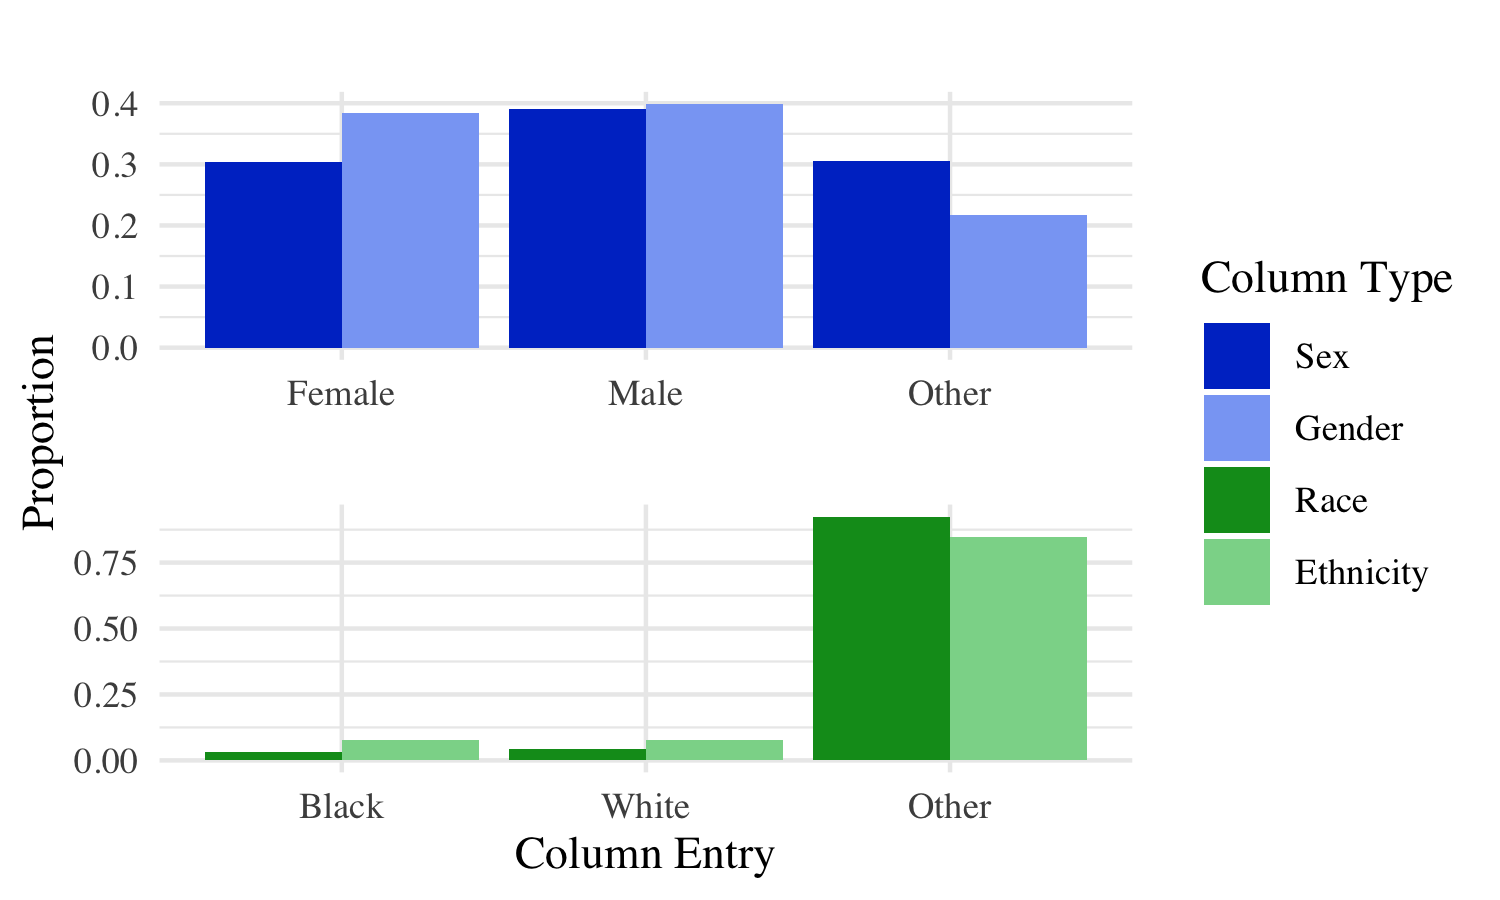
\includegraphics[width=.8\linewidth]{figures/common_entries.png}
    \captionsetup{width=0.8\textwidth}
    \caption*{The proportion of entries in each column type allotted to the most popular entries, or some other entry. The difference in these distributions is tested in evaluating Hypotheses $2(a)$ and $2(b)$. See Tables \ref{tab:n_entries_sex_gender} and \ref{tab:n_entries_race_ethnicity} for raw data.}
    \label{fig:common_entries}
\end{figure}





